\chapter{Pruebas}

En esta sección se abordarán las distintas tareas relacionadas las diferentes pruebas realizadas para asegurar la calidad del producto final antes de su entrega. El  objetivos del proceso de pruebas es la verificación del software; es necesario poner a prueba el comportamiento del software para identificar situaciones en las que no se obtengan los resultados esperados.

\section{Integración continua en el repositorio}

Todas estas pruebas se han ido realizando cada vez que se actualizaba el repositorio del proyecto en GitHub. Para ello, se ha usado \textit{Travis}\footnote{https://travis-ci.org/}, un sistema que permite la integración coninua en nuestro repositorio. Una vez enlazado travis con nuestro repositorio, es un proceso automático que se realizará siempre.

Gracias a esta herramienta libre, se puede comprobar en cualquier momento si el software se encuentra validado o no. En el caso de que el test falle, travis notifica dónde está el error. 

Travis necesita de un archivo de configuración para que él mismo arranque, creando una máquina virtual que simulará el sistema y comenzará a examinar los cambios realizados. Este archivo se llama \textit{.travis.yml}\footnote{https://github.com/guillesiesta/ProjectX/blob/master/.travis.yml} y para que realice los tests para el módulo de la API(python) y de  la interfaz(javascript), se ha tenido que crear el archivo de la manera que muestra la imagen \ref{fig::travis}.

\begin{figure}
    \centerline{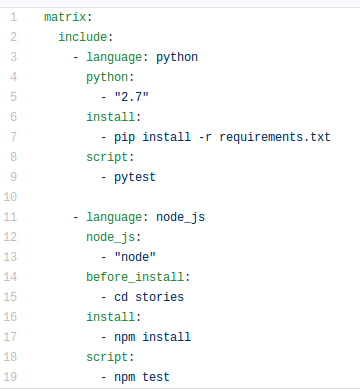
\includegraphics[width=6cm]{figuras/travis.png}}
    \caption{Archivo .travis.yml del repositorio en GitHub}
    \label{fig::travis}
\end{figure}

\section{Pruebas en back-end - API}

Para el correcto funcionamiento de mi API he usado la librería \textit{pytest}\footnote{https://docs.pytest.org/en/latest/} y su plugin para flask\footnote{https://pytest-flask.readthedocs.io/en/latest/}.

Esta herramienta permite la realización de tests unitarios. Por lo que para cada función de mi API he realizado el siguiente testeo:

\begin{itemize}
    \item \textbf{all\_stories\_titulo()}. Cuento todas las historias existentes en la base de datos y guardo esa cantidad. Añado 1 historia y compruebo que las historias existentes son la cantidad anterior más 1.
     \item \textbf{user\_stories\_titulo()}. Creo un acertijo, creo un usuario, creo la relación (usuario)-[escribe]-(acertijo) y compruebo que la historia introducida existe y está escrita por ese usuario.
     \item \textbf{soluciones\_por\_titulo()}. Creo un acertijo y un usuario. Creo la relación (usuario)-[propone solución]-(acertijo) y compruebo que esa solución para ese acertijo existe.
     \item \textbf{enviar\_comentario()}. Creo acertijo y usuario. Creo la relación (usuario)-[propone solución]-(acertijo) y compruebo que esa solución propuesta ha sido añadida en el sistema.
     \item \textbf{enviar\_storie()}. Creo acertijo y usuario, creo la relación (usuario)-[escribe]-(acertijo), y compruebo que ese acertijo tiene todos los campos iguales que el acertijo creado.
     \item \textbf{cambiar\_puntuacion()}. Creo acertijo y usuario. Creo la relación (usuario)-[propone solución]-(acertijo). Cambio la puntuación y compruebo que la puntuación para esa solución propuesta ha sido modificada.
     \item \textbf{acertijo\_por\_titulo()}.Creo un acertijo y compruebo que, buscándolo en la base de datos por su título, éste existe.
     \item \textbf{storie\_por\_titulo()}. Creo un acertijo y compruebo que, buscándolo en la base da datos por su título, la solución a él existe.
     \item \textbf{todo\_por\_titulo()}. Creo un acertijo y compruebo que, a través de su título, lo busco en la base de datos y devuelvo todos sus atributos.
     \item \textbf{login()}. Creo un usuario en el sistema con nombre y contraseña y compruebo que éste ha sido añadido al sistema correctamente.
\end{itemize}

Todos estos tests se materializan en código en el repositorio de GitHub de la aplicación\footnote{https://github.com/guillesiesta/ProjectX/blob/master/stories/test\_storie.py}. 

\section{Pruebas en front-end}

Para testear la interfaz he usado \textit{jest}\footnote{https://jestjs.io/} junto con \textit{enzyme}\footnote{https://github.com/airbnb/enzyme}. Esta recomendación para el testeo viene dada por la propia documentación de ReacJS\cite{testreact}.

La idea principal para las pruebas es comprobar que cada componente creado en ReactJS se renderiza de una manera correcta. Para ello gracias a enzyme, puedo crear un \textit{snapshot} o instantánea de ese componente antes de renderizar, y una vez se renderice, se comprueba que el componente está creado de la manera esperada\cite{testreact2}.

Dicho de otra manera se le dice a Jest que se quiere estar seguro de que la salida de este componente nunca debe cambiar accidentalmente y Jest, con ayuda de enzyme la guarda en un archivo, y después comprueba que el componente no ha sido cambiado una vez se renderice.